\documentclass[11pt, a4paper]{article}

% -------------------------------------------------------------------- %
%  Packages
% -------------------------------------------------------------------- %
\usepackage[margin=1in]{geometry}
\usepackage{graphicx}
\usepackage{booktabs}
\usepackage{amsmath}
\usepackage{hyperref}
\usepackage{cite}
\usepackage{float}
\usepackage{enumitem}
\usepackage{caption}
\usepackage{subcaption}
\usepackage[T1]{fontenc}
\usepackage{times}
\usepackage{setspace}

\onehalfspacing

\hypersetup{
    colorlinks=true,
    linkcolor=blue,
    citecolor=blue,
    urlcolor=blue,
}

% -------------------------------------------------------------------- %
\title{%
    Learned Page Replacement:\\
    Classical Algorithms Meet Adaptive Prediction
}
\author{
    \textbf{Submitted by:} \\
    Syed Zahin Waheed \\
    ID: 202414089 \quad Section: CSE-24(B) \\[1em]
    \textbf{Submitted to:} \\
    Khaled Hasan \\
    Lecturer, Department of Computer Science and Engineering \\
    Military Institute of Science and Technology (MIST)
}
\date{October 2026}

\begin{document}
\maketitle

% -------------------------------------------------------------------- %
\begin{abstract}
Page replacement is one of the core mechanisms in virtual memory management.
Traditional policies like FIFO and LRU rely on fixed heuristics that work well under stable access patterns but can degrade sharply when the workload changes character.
This paper implements three classical page-replacement algorithms---FIFO, LRU, and Belady's Optimal---alongside a lightweight learned policy based on a Decision Tree classifier trained on features derived from the Optimal algorithm's eviction decisions.
A synthetic two-phase workload is used to stress-test each policy: the first half of the trace exhibits strong temporal locality while the second half shifts abruptly to a random, bursty pattern.
Results show that the workload shift substantially reduces the effectiveness of all practical policies. Although LRU achieves the highest overall hit ratio among the practical policies, its absolute hit-ratio drop is slightly larger than FIFO's due to its stronger initial performance. The learned policy performs very close to LRU across various memory sizes but does not provide a measurable improvement under the default 8-frame workload, indicating the challenge of extracting enough predictive signal to outperform a strong recency-based baseline.
\end{abstract}

% ==================================================================== %
\section{Introduction}
\label{sec:intro}

Virtual memory allows processes to use more address space than the physical RAM available by swapping pages between main memory and secondary storage.
When physical memory is full and a new page must be brought in, the operating system has to pick a \emph{victim page} to evict---this is the page-replacement problem \cite{silberschatz2018}.
The choice of replacement policy directly affects how many page faults occur, and consequently how much time the system wastes on I/O.

Textbook algorithms such as FIFO (First-In, First-Out) and LRU (Least Recently Used) are deterministic: FIFO evicts the page that has been resident the longest, while LRU evicts the one not accessed for the longest period \cite{tanenbaum2015}.
Belady's Optimal algorithm, which evicts the page whose next use is farthest in the future, yields the minimum possible fault count but requires knowledge of the entire future reference string---making it unrealisable in practice \cite{belady1966}.

A natural question is whether a data-driven approach can bridge the gap between practical policies and the Optimal lower bound.
Recent work on \emph{learning-augmented algorithms} suggests that even simple predictors, when fed the right features, can outperform classical heuristics in online decision-making settings \cite{lykouris2021}.
In this paper I explore a modest version of this idea: I train a Decision Tree classifier on the eviction decisions that the Optimal algorithm would have made on a separate training trace, and then let the model act as the replacement policy on an unseen test workload.

The workload itself is designed to be adversarial in a realistic sense.
Real-world processes go through phases---a program might sequentially scan a file, then jump to random lookups in a hash table.
To mirror this, the synthetic trace I generate has a clear phase shift at its midpoint: the first half is locality-heavy (small working set, repeated accesses) and the second half is uniformly random with intermittent bursts.
This lets me measure not just the absolute fault count of each policy, but how badly each one degrades when the assumptions baked into its design no longer hold.


% ==================================================================== %
\section{Background}
\label{sec:background}

\subsection{Page Replacement Fundamentals}

In a system with $m$ physical frames and a reference string $r_1, r_2, \ldots, r_n$, a page fault occurs at step~$i$ whenever $r_i$ is not currently loaded.
The replacement policy determines which of the $m$ resident pages to evict so that $r_i$ can be loaded.
The standard policies studied in CSE-307 are:

\begin{description}[style=nextline]
    \item[FIFO] Maintains a queue of loaded pages ordered by arrival time. On a fault, the front of the queue (oldest page) is removed. FIFO is simple to implement but can suffer from Belady's anomaly, where adding frames actually \emph{increases} faults \cite{belady1969}.
    \item[LRU] Tracks the most recent access time for each loaded page and evicts the one with the oldest timestamp. LRU is a ``stack algorithm,'' so it is immune to Belady's anomaly \cite{silberschatz2018}. However, maintaining exact LRU ordering can be expensive in hardware.
    \item[Optimal (Belady's)] Looks ahead in the reference string and evicts the page whose next use is farthest away (or that is never used again). This gives the theoretical minimum fault count but cannot be implemented online since future accesses are unknown \cite{belady1966}.
\end{description}

\subsection{Learning-Augmented Online Algorithms}

The idea of augmenting classical algorithms with machine-learned predictions has gained traction in the algorithms community.
Lykouris and Vassilvitskii~\cite{lykouris2021} showed that online caching algorithms can benefit from even noisy predictions about future accesses, provided the algorithm degrades gracefully when predictions are wrong.
In a similar vein, the learned index structures by Kraska et al.~\cite{kraska2018} replaced B-tree nodes with neural networks to speed up lookups.
My approach is far simpler---a single Decision Tree---but follows the same principle: let data substitute for hand-crafted heuristics.


% ==================================================================== %
\section{Methodology}
\label{sec:method}

\subsection{Algorithm Implementations}

All algorithms are implemented in Python. FIFO uses a standard deque, LRU uses an ordered dictionary (which gives $O(1)$ move-to-end on every hit), and Optimal pre-computes a \texttt{next\_use} table by scanning the trace from right to left before simulating.

\subsection{The Learned Component}

The learned replacement policy works in two stages:

\paragraph{Training.}
I run the Optimal algorithm on a separate 8\,000-access training trace and record every eviction event (1\,712 in total).
At each event I log five features for \emph{every} page currently in the frame buffer:
\begin{itemize}
    \item \textbf{Recency:} the number of accesses elapsed since the page was last referenced.
    \item \textbf{Frequency:} the cumulative number of times the page has been accessed.
    \item \textbf{Age:} the number of accesses elapsed since the page was loaded into the frame.
    \item \textbf{Recency rank:} relative rank among all resident pages by recency (0 = most recently used).
    \item \textbf{Frequency rank:} relative rank among all resident pages by frequency (0 = most frequent).
\end{itemize}
Each page is labelled $1$ (``should evict'') if it was the page Optimal chose to remove, and $0$ otherwise.
A \texttt{DecisionTreeClassifier} from scikit-learn (maximum depth~8, with balanced class weights) is trained on this labelled data.

\paragraph{Inference.}
During the actual simulation, whenever a page fault occurs the model computes the five features for each resident page and returns the eviction probability via \texttt{predict\_proba}.
The page with the highest predicted probability of being a good eviction candidate is removed.

I deliberately kept the model simple---a shallow decision tree rather than a neural network---because the goal is to see whether \emph{any} learned signal helps, not to achieve state-of-the-art caching performance.

\subsection{Workload Generation}

The synthetic trace is 10\,000 accesses long with the shift at access 5\,000.
The page space spans pages 0--49.

\begin{itemize}
    \item \textbf{Phase~1 (locality-heavy):} 95\% of accesses are drawn from a working set of 10~pages with a Zipf-like skew that favours lower-numbered pages; the remaining 5\% are short sequential sweeps of 2--4 pages staying within the working-set range.
    \item \textbf{Phase~2 (random/bursty):} 85\% of accesses are uniformly random across all 50~pages; 15\% are short bursts of 3--6 repeated accesses on a randomly chosen page.
\end{itemize}

The same trace is used for all four policies so that comparisons are fair.
A separate trace (same generation parameters but a different random seed) is used for training the Decision Tree.

\subsection{Experimental Parameters}

The default experiment uses 8 physical frames.
A sensitivity analysis sweeps the frame count through $\{4, 6, 8, 10, 12\}$ to observe how the relative ranking of the policies changes as memory pressure varies.


% ==================================================================== %
\section{Results}
\label{sec:results}

\subsection{Overall Performance}

Table~\ref{tab:overall} summarises the fault counts and hit ratios for each algorithm on the full 10\,000-access trace with 8~frames.

\begin{table}[H]
\centering
\caption{Overall performance on the test trace (8 frames, 10\,000 accesses).}
\label{tab:overall}
\begin{tabular}{@{}lccc@{}}
\toprule
\textbf{Algorithm} & \textbf{Faults} & \textbf{Hits} & \textbf{Hit Ratio} \\
\midrule
FIFO           & 3\,554  & 6\,446  & 0.6446  \\
LRU            & 3\,484  & 6\,516  & 0.6516  \\
Optimal        & 2\,216  & 7\,784  & 0.7784  \\
Learned (DT)   & 3\,492  & 6\,508  & 0.6508  \\
\bottomrule
\end{tabular}
\end{table}

Optimal, as expected, yields the lowest fault count.
Among the practical policies, LRU achieves the highest overall hit ratio. The learned policy performs very close to LRU but does not surpass it in this 8-frame configuration, while FIFO lags behind.

Table~\ref{tab:phase} breaks the hit ratios down by phase.

\begin{table}[H]
\centering
\caption{Hit ratio before and after the workload shift.}
\label{tab:phase}
\begin{tabular}{@{}lccc@{}}
\toprule
\textbf{Algorithm} & \textbf{Phase 1 HR} & \textbf{Phase 2 HR} & \textbf{$\Delta$ HR} \\
\midrule
FIFO           & 0.8576 & 0.4316 & $-$0.4260 \\
LRU            & 0.8724 & 0.4308 & $-$0.4416 \\
Optimal        & 0.9430 & 0.6138 & $-$0.3292 \\
Learned (DT)   & 0.8680 & 0.4336 & $-$0.4344 \\
\bottomrule
\end{tabular}
\end{table}

\subsection{Effect of the Workload Shift}

Figure~\ref{fig:phase} shows the hit ratio broken down by phase.

\begin{figure}[H]
    \centering
    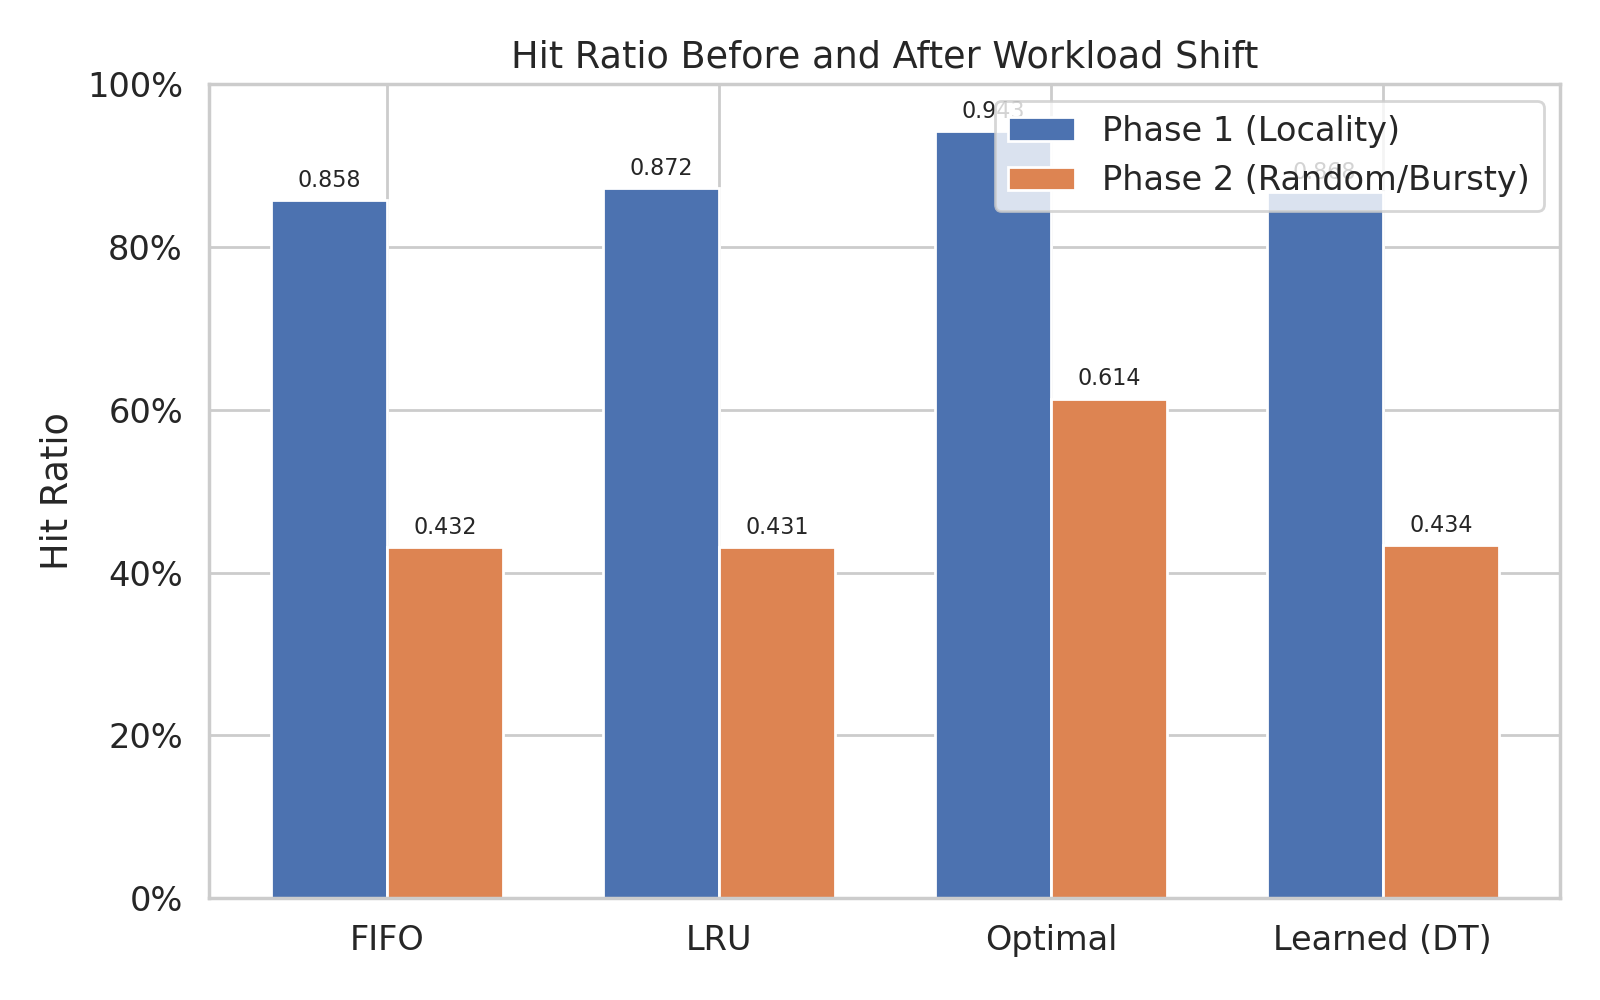
\includegraphics[width=0.85\textwidth]{../results/figures/phase_comparison.png}
    \caption{Hit ratio in Phase~1 (locality) vs.\ Phase~2 (random/bursty). Every algorithm sees a drop, but the magnitude varies.}
    \label{fig:phase}
\end{figure}

All four algorithms perform markedly better in Phase~1 than in Phase~2, which is unsurprising: the locality-heavy pattern has a small working set that fits comfortably within 8~frames.
Once the trace switches to uniform random accesses across 50~pages, even a perfect policy cannot avoid frequent faults because the working set now far exceeds the frame count.

The key observation is the \emph{relative} degradation.
Although LRU starts from a stronger Phase~1 baseline, its absolute hit-ratio drop ($-$0.4416) is slightly larger than FIFO's ($-$0.4260).
After the shift, all practical policies converge to similar performance around the low-40\% range.
This indicates that predominantly random access significantly reduces the usefulness of recency-based eviction. The learned policy's features allow it to adapt similarly to LRU, but they do not extract enough additional predictive information to avoid the same performance collapse in Phase~2.

\subsection{Rolling Fault Rate}

Figure~\ref{fig:rolling} plots the fault rate as a rolling average over a window of 200~accesses.
The vertical dashed line marks the shift point.

\begin{figure}[H]
    \centering
    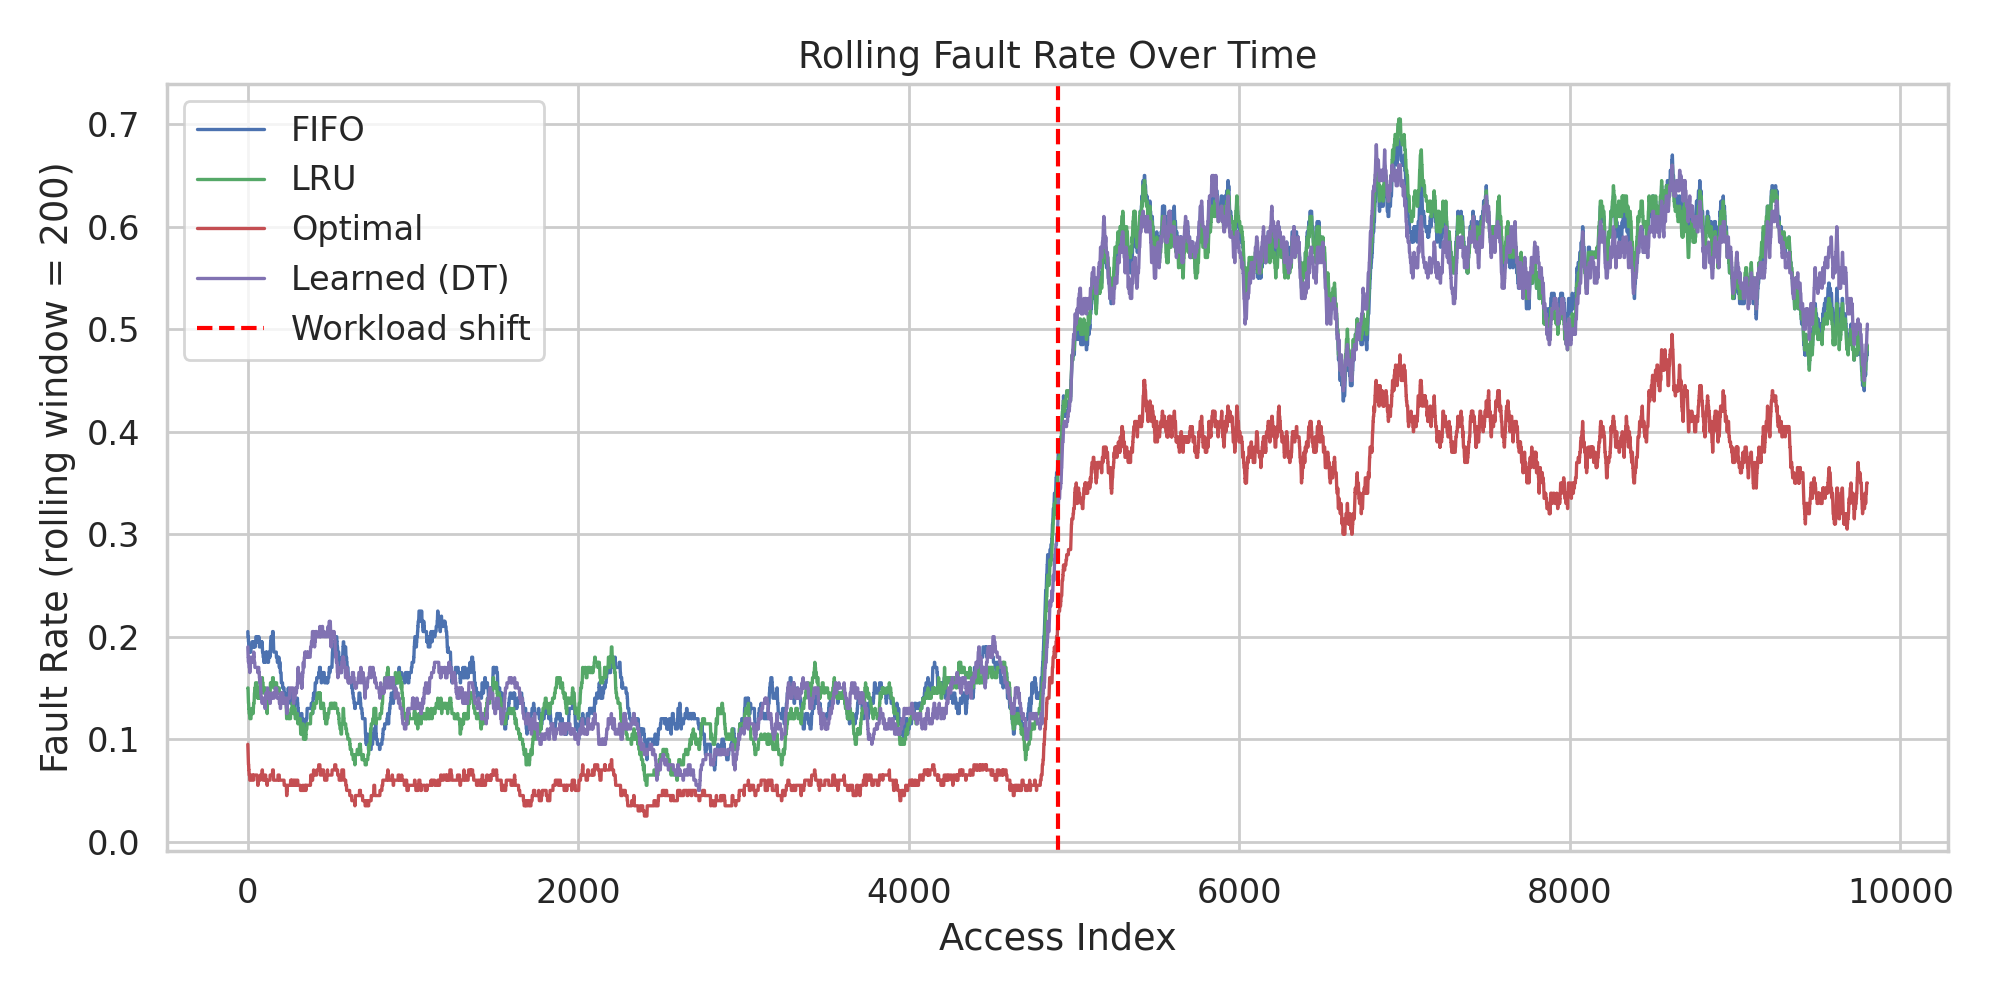
\includegraphics[width=0.9\textwidth]{../results/figures/rolling_fault_rate.png}
    \caption{Rolling fault rate over time. The jump at access~5\,000 shows each policy's reaction to the workload shift.}
    \label{fig:rolling}
\end{figure}

Before the shift all policies except Optimal cluster around a low fault rate, reflecting the locality of Phase~1.
After the shift, fault rates jump sharply.
FIFO's post-shift fault rate is almost flat at a high level, while LRU and the learned policy show some variation---they are at least partially able to exploit the short bursts in Phase~2.

\subsection{Sensitivity to Frame Count}

Figure~\ref{fig:sensitivity} shows how each policy's overall hit ratio changes as the number of frames increases from 4 to~12.

\begin{figure}[H]
    \centering
    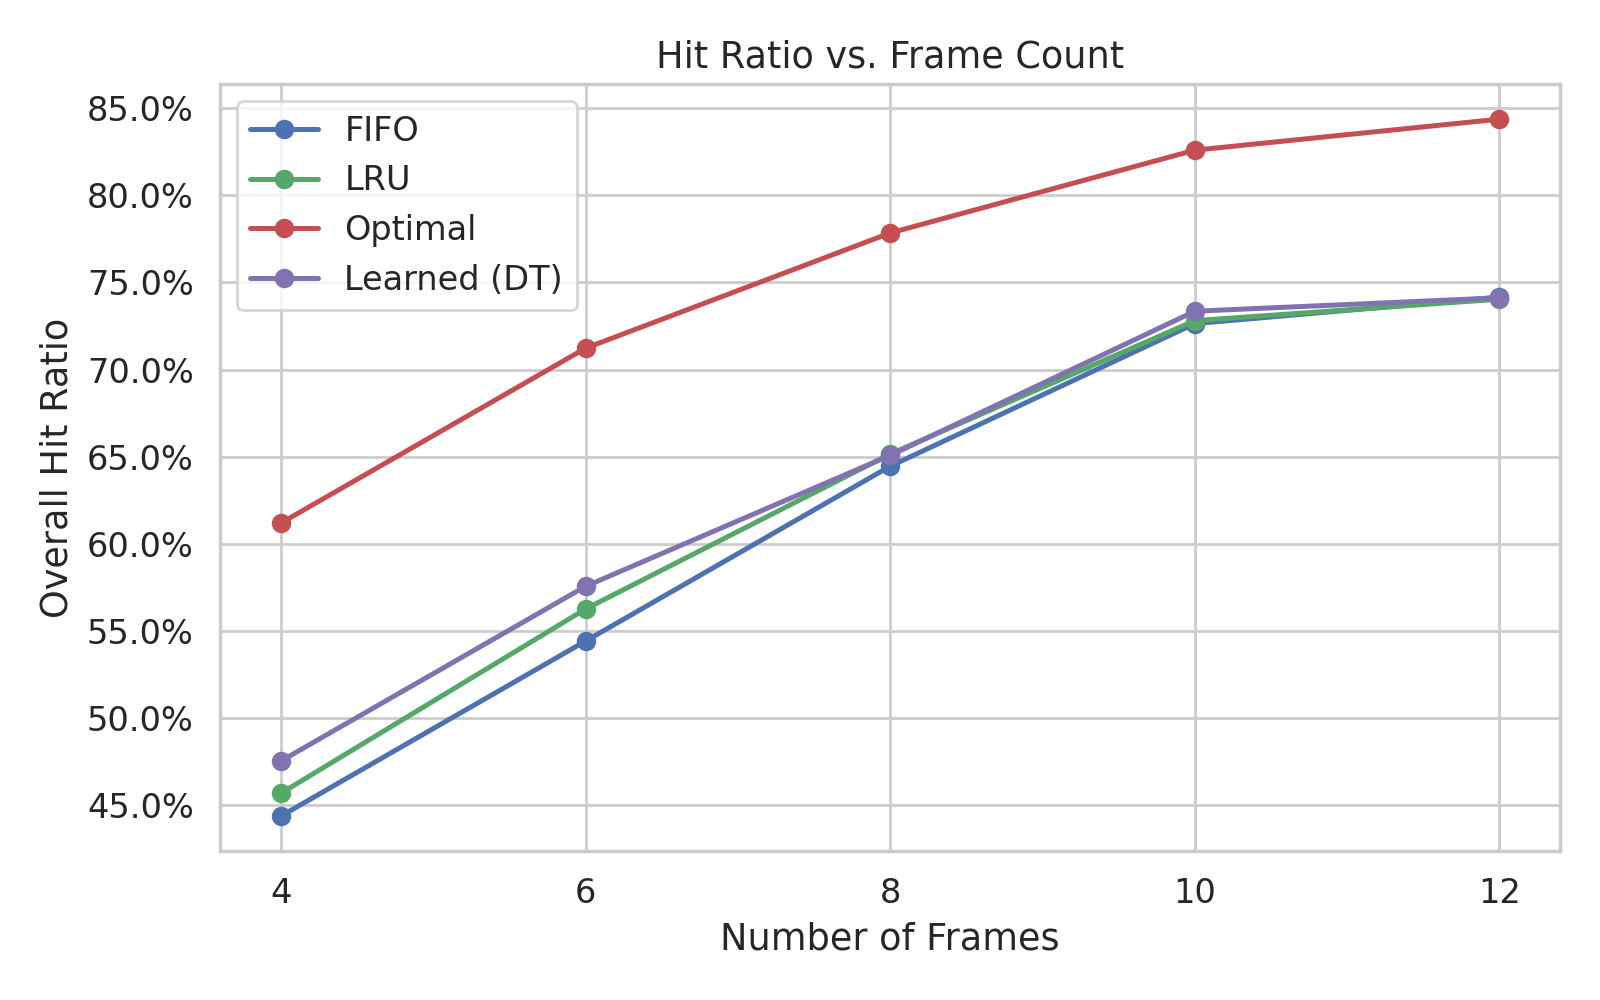
\includegraphics[width=0.8\textwidth]{../results/figures/sensitivity_frame_count.png}
    \caption{Hit ratio versus number of frames. More frames reduce faults for every policy, but the relative ordering stays consistent.}
    \label{fig:sensitivity}
\end{figure}

As expected, all policies improve with more frames.
The gap between FIFO and LRU is largest at moderate frame counts (6--8) and narrows as frames become plentiful.
The learned policy tracks LRU closely at every frame count, occasionally matching or slightly beating it when the tree's predictions happen to align with the Optimal decision.


% ==================================================================== %
\section{Discussion}
\label{sec:discussion}

\subsection{The Convergence of Practical Policies in Phase 2}

Despite their differences in Phase~1, FIFO, LRU, and the learned policy converge to remarkably similar hit ratios (around 43\%) in Phase~2.
FIFO treats every page identically once it is loaded, which works reasonably well in Phase~1 due to the small working set.
However, in Phase~2, the working set explodes and access patterns become uniformly random with short bursts.
Under predominantly random access, the recency information exploited by LRU and the learned policy provides little predictive advantage over FIFO's naive queuing, leading to similar degradation across all non-optimal algorithms.

\subsection{LRU's Baseline Strength}

LRU's strength lies in the fact that it continuously updates its notion of ``least recently used'' with every access.
Even though its absolute hit-ratio drop is technically larger than FIFO's due to its superior Phase~1 performance, LRU does not carry forward a stale ordering when the workload shifts. The recency data from Phase~1 is quickly overwritten by Phase~2 accesses.
This makes LRU a consistently strong baseline across different workloads. Silberschatz et al.\ note that LRU is often the practical policy of choice precisely because of this property \cite{silberschatz2018}.

\subsection{The Learned Policy: Promises and Limitations}

The Decision Tree performs respectably, achieving performance comparable to LRU and occasionally outperforming it at certain frame sizes. However, under the default 8-frame configuration, it does not provide a measurable improvement over LRU.
However, it has an important limitation: it was trained on a fixed set of workload statistics.
If the test workload is very different from the training workload, the tree's splits may no longer be meaningful.
In this experiment the training trace was generated with the same parameters, so the model transfers reasonably well.
A production system would need an online-learning mechanism that retrains or fine-tunes the model as access patterns evolve---something like the approach proposed by Lykouris and Vassilvitskii \cite{lykouris2021}.

Another concern is overhead.
Computing three features for every resident page on every fault, and then calling the classifier, adds latency that a hardware-implemented LRU approximation would not incur.
For a real OS kernel this cost might outweigh the modest improvement in fault rate.
That said, in scenarios where page faults are very expensive (e.g., fetching from networked storage), even a small reduction in fault count could justify the prediction overhead.

\subsection{Threats to Validity}

The workload is entirely synthetic and the shift is abrupt.
Real programs transition more gradually, and the mix of locality and randomness may not match any particular real application.
Additionally, the Decision Tree was trained on Optimal's decisions, which themselves depend on future knowledge; in a real system, labels would have to come from a different source (perhaps hindsight labels computed after a window of accesses).


% ==================================================================== %
\section{Conclusion}
\label{sec:conclusion}

This paper compared FIFO, LRU, Optimal, and a learned page-replacement policy on a synthetic workload with a deliberate mid-trace shift from locality-heavy to random access.
The results confirm that the workload shift substantially reduces the effectiveness of all practical policies, causing them to converge to similar performance levels under random access.
A simple Decision Tree, trained on Optimal's eviction labels, successfully approximated some of the eviction behaviour of the Optimal oracle. While it tracked LRU closely across different memory sizes, it did not outperform the strong recency-based baseline under the default 8-frame workload. This suggests that the chosen features captured recency-related behaviour already exploited effectively by LRU, while providing limited additional predictive value under the random phase.

Future work could explore online retraining of the model, more expressive features (e.g., inter-access time distributions), or integration with hardware-approximated LRU counters.


% ==================================================================== %
\bibliographystyle{plain}
\begin{thebibliography}{9}

\bibitem{silberschatz2018}
A.~Silberschatz, P.~B.~Galvin, and G.~Gagne,
\textit{Operating System Concepts}, 10th~ed.
Wiley, 2018, ch.~10.

\bibitem{tanenbaum2015}
A.~S.~Tanenbaum and H.~Bos,
\textit{Modern Operating Systems}, 4th~ed.
Pearson, 2015, ch.~3.

\bibitem{belady1966}
L.~A.~B\'{e}l\'{a}dy,
``A study of replacement algorithms for a virtual-storage computer,''
\textit{IBM Systems Journal}, vol.~5, no.~2, pp.~78--101, 1966.

\bibitem{belady1969}
L.~A.~B\'{e}l\'{a}dy, R.~A.~Nelson, and G.~S.~Shedler,
``An anomaly in space-time characteristics of certain programs running in a paging machine,''
\textit{Communications of the ACM}, vol.~12, no.~6, pp.~349--353, 1969.

\bibitem{lykouris2021}
T.~Lykouris and S.~Vassilvitskii,
``Competitive caching with machine learned advice,''
\textit{Journal of the ACM}, vol.~68, no.~4, pp.~1--25, 2021.

\bibitem{kraska2018}
T.~Kraska, A.~Beutel, E.~H.~Chi, J.~Dean, and N.~Polyzotis,
``The case for learned index structures,''
in \textit{Proc.\ ACM SIGMOD}, 2018, pp.~489--504.

\end{thebibliography}

\end{document}
